\documentclass[a4paper, 12pt, twoside]{report}
\usepackage[utf8]{inputenc}
\usepackage[T1]{fontenc}
\usepackage[english]{babel}
\usepackage{lmodern}
\usepackage[top=2.5cm, bottom=2cm,
			left=3cm, right=2.5cm,
			headheight=15pt]{geometry}
\usepackage{graphicx}
\usepackage{eso-pic}
\usepackage{array}
\usepackage{longtable}
\usepackage{xcolor}
\usepackage{tikz}
\usetikzlibrary{arrows.meta,positioning,shapes.geometric,calc}
\usepackage{pgfplots}
\pgfplotsset{compat=1.18}
\usepackage{hyperref}
\usepackage{lastpage}
\definecolor{bleuleger}{RGB}{0,0,200}

\usepackage{listings}
\lstnewenvironment{codeC}[1][]
{%
	\lstset{language=C,
		frame=single,
		captionpos=b,
		backgroundcolor=\color{bleuleger!5},
		basicstyle=\ttfamily\tiny,
		numbers=left,
		numberstyle=\color{black},
		numbersep=5pt,
		breaklines=true,
		tabsize=4,
		keywordstyle=\bfseries\color{green!40!black},
		stringstyle=\color{red}\ttfamily,
		identifierstyle=\color{blue},
		caption={[#1]{#1}},
		commentstyle=\color{purple!40!black}}
}
{}
%%%%%%%%%%%%%%%%%%%%%%%%%%%%%%%%%%%%%%%%
%    Page de garde (Pagedegarde.tex)   %
%%%%%%%%%%%%%%%%%%%%%%%%%%%%%%%%%%%%%%%%
% Dorian Depriester, 2014
\usepackage{fancyhdr}
\usepackage{nomencl}
\makeatletter
\def\@ecole{School}
\newcommand{\ecole}[1]{
  \def\@ecole{#1}
}

\def\@entreprise{Company name}
\newcommand{\entreprise}[1]{
  \def\@entreprise{#1}
}

\def\@datedebut{\today}
\newcommand{\datedebut}[1]{
  \def\@datedebut{#1}
}


\def\@datefin{\today}
\newcommand{\datefin}[1]{
  \def\@datefin{#1}
}



\def\@specialite{Specialization}
\newcommand{\specialite}[1]{
  \def\@specialite{#1}
}

\def\@ED{Graduate school}
\newcommand{\ED}[1]{
  \def\@ED{#1}
}

\def\@doctorat{Doctorat}
\newcommand{\doctorat}[1]{
  \def\@doctorat{#1}
}

\def\@adresse{Address}
\newcommand{\adresse}[1]{
  \def\@adresse{#1}
}

\def\@directeur{Supervisor}
\newcommand{\directeur}[1]{
  \def\@directeur{#1}
}

\def\@fonction{Role}
\newcommand{\fonction}[1]{
  \def\@fonction{#1}
}

\def\@encadrant{Mentor}
\newcommand{\encadrant}[1]{
  \def\@encadrant{#1}
}
\def\@jurya{}{}{}
\newcommand{\jurya}[3]{
  \def\@jurya{#1,	& #2	& #3\\}
}
\def\@juryb{}{}{}
\newcommand{\juryb}[3]{
  \def\@juryb{#1,	& #2	& #3\\}
}
\def\@juryc{}{}{}
\newcommand{\juryc}[3]{
  \def\@juryc{#1,	& #2	& #3\\}
}
\def\@juryd{}{}{}
\newcommand{\juryd}[3]{
  \def\@juryd{#1,	& #2	& #3\\}
}
\def\@jurye{}{}{}
\newcommand{\jurye}[3]{
  \def\@jurye{#1,	& #2	& #3\\}
}
\def\@juryf{}{}{}
\newcommand{\juryf}[3]{
  \def\@juryf{#1,	& #2	& #3\\}
}
\def\@juryg{}{}{}
\newcommand{\juryg}[3]{
  \def\@juryg{#1,	& #2	& #3\\}
}
\def\@juryh{}{}{}
\newcommand{\juryh}[3]{
  \def\@juryh{#1,	& #2	& #3\\}
}
\def\@juryi{}{}{}
\newcommand{\juryi}[3]{
  \def\@juryi{#1,	& #2	& #3\\}
}
\makeatother

\newcommand\BackgroundPic{%
	\put(0,0){%
		\parbox[b][\paperheight]{\paperwidth}{%
			
\includegraphics[height=0.45\paperheight]{Bordure.png}%
			\vfill
		}
	}
}
\newcommand\EtiquetteThese{%
	\put(0,0){%
		\parbox[t][\paperheight]{\paperwidth}{%
			\hfill
			%\colorbox{blue}{		
				\begin{minipage}[b]{2em}
					
\includegraphics[width=4.0\textwidth]{logo_miage.png}\\					
					%\centering\Huge\textcolor{white}{M\\I\\A\\G\\E\\}
					\vspace{0.2cm}
				\end{minipage}
			%}
		}
	}
}

\makeatletter
\newcommand{\pagedegarde}{
\newgeometry{top=2.5cm, bottom=1cm, left=2cm, right=1cm}
\AddToShipoutPicture*{\BackgroundPic}
%\AddToShipoutPicture*{\EtiquetteThese}
  \begin{titlepage}
  \centering
      
\includegraphics[width=0.6\textwidth]{logo_Paris_Nanterre_couleur_RVB.png}
      \hfill
      
\includegraphics[width=0.20\textwidth]{logo_entreprise.png}\\
    \vspace{1cm}
     % {\Large Licence MIASHS parcours MIAGE}\\
    \vspace{1cm}
      {\huge 
      	{\bfseries M1 thesis}\\
    \vspace{0.5cm}}
      	Master MIAGE (apprenticeship)\\
    \vspace{1cm}
   		
    \vspace{1cm}
    	{\huge\color[rgb]{0,0,1} \bfseries{\@title}}\\
    \vspace{0.5cm}
    {\bfseries Host organization: \@entreprise}\\
    {\bfseries Thesis period: \@datedebut\ -- \@datefin}\\
    %	{\Large{\bfseries Spécialité doctorale ``\@specialite''}}\\
    \vspace{2cm}
    	\textit{Presented and defended by}\\
    \vspace{0.5cm}
    	{\Large {\bfseries \@author}} \\
    \vspace{0.5cm}
    	\@date \\
    \vfill
     %  {\LARGE \color[rgb]{0,0,1} \bfseries{\@title}} \\
    %\vfill
      %  Directeur de thèse : {\bfseries \@directeur}\\
       % Co-encadrant de thèse : {\bfseries \@encadrant}\\
    %\vfill
	\begin{tabular}{>{\bfseries}lll}
		\large Defense committee\\
		\vspace{0.15cm}\\
		\@jurya
		\@juryb
		\@juryc
		%\@juryd
		%\@jurye
		%\@juryf
		%\@juryg
		%\@juryh
		%\@juryi
	\end{tabular}
	%
\includegraphics[width=0.20\textwidth]{logo_entreprise.png}\
	\vfill
	
	%\@adresse
  \end{titlepage}




\restoregeometry  
\makenomenclature

\pagestyle{fancy}

\renewcommand\headrulewidth{1pt}

\fancyhead[L]{\@fonction}

\fancyhead[R]{\@entreprise}


\renewcommand\footrulewidth{1pt}

\fancyfoot[L]{\@author}

\fancyfoot[C]{}

\fancyfoot[R]{Page \thepage/\pageref{LastPage}}
}


\author{Seyed Amineddin MIRI}
\title{A Systematic Mapping Study of Learned Indexes in Database Systems}
\entreprise{Agiga}
\fonction{Full Stack Developer}
\datedebut{May 4, 2026}
\datefin{May 31, 2026}

\date{June 16, 2026}
\jurya{M. François Delbot}{Maître de conférences}{Responsable du master}
\juryb{M. Pascal Poizat}{Professeur des universités}{Tuteur enseignant}
\juryc{M. Nicolas Loriot}{CTO}{Maître d'apprentissage}

\begin{document}
\pagedegarde

\chapter*{Acknowledgments}
I would like to express my sincere gratitude to my academic tutor, Professor Pascal Poizat, for his guidance, availability, and methodological advice throughout the preparation of this thesis. His feedback helped me structure the work and keep a rigorous approach to the systematic mapping study.

I also thank Mr. François Delbot, Maître de conférences and head of the master's program, for his supervision of the M1 thesis framework and for the scientific writing guidelines provided during the year. These guidelines were particularly useful in organizing the document and clarifying the expected academic standards.

I am grateful to Mr. Nicolas Loriot, CTO at Agiga and my apprenticeship supervisor, for his trust, support, and the professional environment he provided during this year. Even though the thesis work was conducted independently, my experience at Agiga helped me develop the technical maturity and discipline needed to complete it.

I would also like to thank all my colleagues at Agiga for their welcome, their kindness, and the constructive working atmosphere they created. Their daily support made this apprenticeship year both valuable and motivating.

Finally, I thank my family, my friends, and the people who supported me during the writing of this thesis. Their encouragement, patience, and help during this period were very important to me.

\chapter*{Abstracts}
\section*{Résumé}
Les index de bases de données jouent un rôle central dans les performances des SGBD, mais leur efficacité dépend fortement de la distribution des données, du type de requêtes, de la mémoire disponible, du stockage et des mises à jour. Les index appris, ou learned indexes, ont introduit l'idée de modéliser la relation entre les clés et leurs positions dans des données ordonnées, avec la promesse de structures d'accès plus compactes ou plus rapides dans certains contextes favorables. Depuis cette proposition, la littérature s'est élargie : elle comprend désormais des structures d'index, des benchmarks, des index modifiables, des méthodes de réglage, des analyses de robustesse et les premières intégrations dans des moteurs de stockage ou des SGBD.

Ce mémoire présente une étude de cartographie systématique des index appris dans les systèmes de bases de données. L'étude part de cinq articles représentatifs, analyse les références citées et les articles qui les citent, puis complète ce processus par une recherche ciblée sur les travaux liés au stockage disque, aux moteurs de stockage et à l'intégration dans les SGBD. Le corpus final comprend 18 études primaires, classées selon leur type de contribution, leur famille d'index, les charges de travail et contextes système étudiés, les pratiques d'évaluation et les éléments de reproductibilité disponibles. La cartographie montre une forte couverture des index unidimensionnels sur clés ordonnées, en particulier pour les recherches ponctuelles et les requêtes par intervalle, avec une attention croissante aux insertions, aux charges mixtes et à la robustesse. Elle met aussi en évidence des preuves plus limitées pour les accès concurrents, les longues séquences de mises à jour, l'exécution sur disque, les environnements dépassant la mémoire principale et l'intégration complète dans les SGBD. Dans l'ensemble, les index appris apparaissent comme un espace de conception prometteur mais dépendant des conditions d'utilisation : les résultats les plus solides concernent encore des charges de travail ciblées en mémoire, tandis que l'évaluation robuste, reproductible et intégrée au niveau système reste le principal défi pour les travaux futurs.

\section*{Abstract}
Database indexes are central to DBMS performance, yet their effectiveness depends heavily on data distribution, workload, memory, storage, and update patterns. Learned indexes introduced the idea of modeling the relationship between keys and positions in ordered data, promising smaller or faster access structures in favorable settings. Since that proposal, the literature has expanded from standalone learned structures to benchmarks, updatable designs, tuning methods, robustness analyses, and early integrations into storage engines and DBMSs.

This thesis presents a Systematic Mapping Study of learned indexes in database-system contexts. The study starts from five representative seed papers, applies backward and forward snowballing, and complements this process with a targeted search for disk-resident, storage-engine, and DBMS-integration work. The final corpus contains 18 primary studies, classified by publication and contribution type, index family, workload and system setting, evaluation practice, and reproducibility evidence. The map shows strong coverage of one-dimensional ordered-key indexing, especially lookup and range-query workloads, with increasing attention to inserts, mixed workloads, and robustness. It also reveals thinner evidence for concurrency, long-running updates, disk-resident execution, larger-than-memory settings, and full DBMS integration. Overall, learned indexes appear as a promising but condition-dependent design space: their strongest evidence remains in selected in-memory workloads, while robust, reproducible, system-level evaluation is still the main challenge for future work.

\tableofcontents

\chapter{Introduction}

Database indexes are central components of data management systems. They reduce access cost by avoiding full scans and by organizing or locating records through auxiliary structures such as B+-trees, hash indexes, radix trees, and related access methods. Their effectiveness is not absolute: the preferred indexing strategy depends on the query type, the key distribution, the data volume, the memory budget, the read/write ratio, the storage setting, and the need for concurrent access. This is visible in the learned-index literature itself, where B+-trees, Adaptive Radix Trees, hash-based structures, binary search variants, and specialized learned indexes are repeatedly compared under different workloads and hardware conditions \cite{kraska2018,marcus2020benchmarking,sun2023learned}.

The idea of learned indexes was popularized by Kraska et al., who proposed to view indexes as models: a range index can be interpreted as predicting the position of a key in a sorted array, and this prediction can be learned from the key distribution \cite{kraska2018}. In this view, a learned index approximates the key-to-position mapping, often related to the cumulative distribution function (CDF) of the data. Because model predictions are imperfect, learned indexes must also provide a correction mechanism, such as searching around the predicted position or maintaining error bounds \cite{kraska2018,ding2020alex,sun2023learned,maltry2022critical}.

Since the initial Recursive Model Index proposal, the field has diversified substantially. Some studies propose new learned-index structures, such as FITing-Tree, ALEX, CARMI, the PGM-index, RadixSpline, DILI, and SWIX \cite{galakatos2019fiting,ding2020alex,zhang2022carmi,ferragina2020pgm,kipf2020radixspline,li2023dili,liang2024swix}. Other papers focus on benchmarking, critical analysis, robustness, or practical limitations \cite{marcus2020benchmarking,maltry2022critical,wongkham2022ready,sun2023learned,luo2025robustness}. More recent work also explores disk-resident settings, larger-than-memory storage engines, learned-index tuning, and integration into existing systems such as PostgreSQL or LeanStore \cite{lan2023disk,chatterjee2024limousine,wang2025tuning,fuad2026postlearn,maharjan2023learnedstore}.

This diversification makes the area difficult to summarize through a conventional narrative literature review. Learned-index papers do not all answer the same question: some optimize lookup latency, some study update support, some examine robustness, some provide benchmark infrastructure, and others investigate system integration. In addition, the results are highly conditioned by workload, data distribution, baseline choice, and evaluation setup. For example, benchmark and critical-analysis papers show that learned indexes may be promising under some read-heavy or distribution-friendly settings, while remaining difficult to generalize to write-heavy, concurrent, disk-resident, or complex-distribution scenarios \cite{marcus2020benchmarking,sun2023learned,wongkham2022ready,lan2023disk,luo2025robustness}.

Existing secondary studies already discuss learned indexes, including a general narrative survey and two surveys focused on multi-dimensional learned indexes \cite{faraj2024survey,liu2025multidimensional,almamun2025survey}. These works are used as contextual related work; the present thesis instead maps primary learned-index studies through an explicit SMS protocol.

The remaining gap is therefore not the absence of learned-index surveys, but the absence of a systematic map focused on how primary learned-index studies are distributed and evaluated in database-system contexts. This thesis addresses that gap by conducting a Systematic Mapping Study (SMS). The objective is not to determine which learned index is universally best, nor to design a new index advisor or DBMS architecture. Instead, the objective is to classify the literature according to publication and contribution types, learned-index techniques, workload scenarios, system settings, evaluation practices, and reproducibility evidence.

The study is guided by three research questions:

\begin{itemize}
\item \textbf{RQ1.} What types of learned-index studies have been published, and how are they distributed over time and publication venues?
\item \textbf{RQ2.} Which learned-index techniques and database workload scenarios are addressed in the literature?
\item \textbf{RQ3.} How are learned indexes evaluated, and what evidence is available regarding performance, robustness, and reproducibility?
\end{itemize}

The contribution of the thesis is therefore a structured map of the selected corpus. It identifies the main research clusters, the workload and system settings covered by the literature, the evaluation dimensions used by primary studies, and the gaps that remain visible from a database-systems perspective. The rest of the document is organized as follows. Chapter~2 introduces the technical background needed to understand learned indexes and their evaluation. Chapter~3 presents the SMS methodology. Chapter~4 presents the extracted data and answers the research questions. Chapter~5 interprets the main trends and gaps, and Chapter~6 summarizes the findings and limitations.

\chapter{Background}

This chapter introduces the technical concepts required to understand the mapping study. It does not aim to provide a complete survey of learned indexes. Instead, it defines the vocabulary used later to classify the corpus: traditional indexes and workloads, the learned-index idea, major learned-index families, system settings, and evaluation dimensions.

\section{Database Indexes and Workloads}

An index is an access structure used to locate records without scanning an entire dataset. In the context of sorted data, a range index can be interpreted as a mechanism that maps a lookup key to the position of the first record whose key is equal to or greater than the lookup key \cite{kraska2018}. ALEX's background section describes a B+-tree as a height-balanced range-index structure whose leaf level stores data or pointers in sorted order to facilitate range queries; a lookup traverses to a leaf and then searches within that leaf \cite{ding2020alex}. Kraska et al. contrast this with hash maps, which they describe as strong structures for single-key lookups and as models that map a key to a position in an unsorted array \cite{kraska2018}. Radix and trie-like structures, such as Adaptive Radix Trees, are also common baselines in learned-index evaluations, especially for in-memory lookup workloads \cite{marcus2020benchmarking,sun2023learned}.

Index behavior depends strongly on the workload. A point lookup asks for one key, while a range query asks for all records between two keys. Insert, update, and delete operations require the index to change as the data changes. Bulk loading builds an index from a batch of sorted or unsorted data. Concurrent workloads add another dimension because multiple operations may access or modify the index at the same time. These workload categories are important in learned-index research because many early learned indexes were designed for static or read-only settings, whereas later work studies inserts, deletes, mixed workloads, concurrency, and streaming or sliding-window data \cite{ding2020alex,sun2023learned,wongkham2022ready,liang2024swix}.

\section{The Learned-Index Idea}

Learned indexes start from the observation that an index can be seen as a model. Kraska et al. describe a B-tree-style range index as a structure that predicts the location of a value within a key-sorted set \cite{kraska2018}. A learned index makes this idea explicit by training a model to approximate the mapping from keys to positions. For a sorted array, this mapping is closely related to the cumulative distribution function (CDF) of the keys: if the distribution is known or well approximated, the position of a key can be predicted from the fraction of keys that are smaller than it \cite{kraska2018,marcus2020benchmarking}.

The basic lookup process has two phases. First, the model performs position inference by predicting where a key should appear. Second, because the model may be wrong, the index performs position refinement or error correction by searching around the predicted position or within a predicted error range \cite{sun2023learned,maltry2022critical}. Binary search is a common correction method, but it is not the only possible one: Maltry and Dittrich distinguish standard binary search from model-biased binary search, model-biased linear search, and model-biased exponential search when analyzing RMI configurations \cite{maltry2022critical}. This correction step is essential: learned indexes do not remove the need for exactness, they use a model to reduce the search space.

The original learned-index proposal introduced the Recursive Model Index (RMI), a hierarchy of models in which higher-level models select lower-level models, and leaf-level models predict positions in the data array \cite{kraska2018}. ALEX explains the RMI intuition as replacing internal B+-tree traversal with model inference while still requiring a final search around the predicted position when the model is imperfect \cite{ding2020alex}. This distinction is useful background vocabulary for understanding learned-index lookup, but the mapping itself classifies papers at a higher level, through index family, workload, system setting, and evaluation evidence.

\section{Learned-Index Families}

The corpus contains several families of learned indexes. RMI-style learned indexes use a hierarchy of models to route keys toward more specialized models. This family starts from the original learned-index proposal and remains a reference point in later evaluations and critical analyses \cite{kraska2018,maltry2022critical,sun2023learned}.

Piecewise linear learned indexes approximate the key-to-position mapping by dividing the data distribution into segments and fitting simple models to each segment. FITing-Tree uses bounded-error piecewise linear segments and an upper-level structure to navigate them, exposing a tradeoff between lookup performance and memory footprint \cite{galakatos2019fiting}. The PGM-index also relies on piecewise linear models, with explicit worst-case error bounds and compressed variants \cite{ferragina2020pgm}. RadixSpline combines spline points with a radix table and emphasizes single-pass construction, which is relevant for write-once/read-many and storage-engine-inspired settings \cite{kipf2020radixspline}.

Adaptive and updatable learned indexes address the limitation that static learned indexes do not naturally support changing data. ALEX combines model-based navigation with gapped arrays, model-based inserts, and adaptive node expansion or splitting to support point lookups, range queries, inserts, updates, deletes, and bulk loading in memory \cite{ding2020alex}. CARMI introduces a cache-aware learned-index framework with cost-based construction and multiple node types \cite{zhang2022carmi}. DILI and SWIX further illustrate the expansion of learned-index research toward distribution-driven design and sliding-window workloads \cite{li2023dili,liang2024swix}.

The term ``hybrid'' is used narrowly. In this thesis, a design is treated as hybrid learned/classical only when a learned component is explicitly combined with, selects among, or falls back to a classical index or storage-engine component. This applies most clearly to LearnedStore, where a learned model accelerates LeanStore's B+-tree search while preserving the original B+-tree path as a fallback \cite{maharjan2023learnedstore}. Limousine also fits this narrower sense because it explores learned and classical components inside larger-than-memory cloud storage-engine designs \cite{chatterjee2024limousine}.

\section{System Settings}

System setting is a major distinction in the mapping. Many learned-index studies evaluate indexes as standalone in-memory structures over one-dimensional sorted keys \cite{marcus2020benchmarking,sun2023learned,wongkham2022ready}. This setting is useful for isolating the index structure, but it does not capture all the costs of integration into a DBMS, such as persistence, buffer management, logging, query execution overhead, recovery, or optimizer interaction \cite{fuad2026postlearn}.

Several papers therefore study settings beyond standalone in-memory lookup. Lan et al. evaluate updatable learned indexes in disk-resident DBMS-like settings and show that adapting in-memory learned indexes to disk-resident environments raises additional design constraints \cite{lan2023disk}. Limousine studies larger-than-memory cloud storage-engine design by blending learned and classical components \cite{chatterjee2024limousine}. PostLearn integrates an ALEX-derived learned index into PostgreSQL as an index access method, while LearnedStore integrates a learned model into LeanStore as an accelerator for B+-tree search \cite{fuad2026postlearn,maharjan2023learnedstore}. Outside the primary corpus, SageDB provides broader context for learned and other instance-optimized components inside database systems \cite{ding2022sagedb}.

\section{Evaluation Dimensions}

Evaluation practice is central to this SMS because learned-index claims depend strongly on experimental conditions. The corpus commonly reports lookup latency, throughput, memory footprint, build or training time, update cost, range-query cost, and sometimes microarchitectural measurements such as cache misses or branch behavior \cite{marcus2020benchmarking}. Benchmarking Learned Indexes emphasizes that no single metric fully explains index performance, and that learned and traditional indexes should be compared using common datasets, strong baselines, and multiple dimensions \cite{marcus2020benchmarking}.

Baselines are also important. Benchmarking papers frequently compare against B+-trees, Adaptive Radix Trees, binary search variants, hash-based structures, FAST, and other learned indexes \cite{marcus2020benchmarking,sun2023learned,maltry2022critical}. Dataset choice matters as well: synthetic or simple distributions can make the key-to-position mapping easier to learn, while harder real-world datasets may contain outliers, skew, or irregularities that reduce the advantage of learned models \cite{marcus2020benchmarking}.

Later evaluations broaden the evidence beyond read-only lookup. Sun et al. compare learned indexes across lookup, range, insert, delete, concurrent, and bulk-loading scenarios \cite{sun2023learned}. Wongkham et al. and Luo et al. study robustness under dynamic and concurrent workloads \cite{wongkham2022ready,luo2025robustness}. Lan et al. examine disk-resident behavior, while PostLearn and LearnedStore show that DBMS or storage-engine integration can expose overheads invisible in standalone microbenchmarks \cite{lan2023disk,fuad2026postlearn,maharjan2023learnedstore}.

Reproducibility is another evaluation dimension used in the mapping. Some studies provide public code, datasets, or benchmark frameworks, such as SOSD-style resources and later benchmark artifacts \cite{marcus2020benchmarking,sun2023learned,wongkham2022ready}. Others provide enough implementation details to understand the design but less complete artifact support. The extraction grid therefore records code availability, dataset availability, and reproducibility notes under RQ3.

\chapter{Methodology}

This chapter describes the protocol used to construct and analyze the literature corpus. The study follows the systematic mapping process introduced by Petersen et al.: define research questions, identify relevant papers, screen papers, build a classification scheme, extract data, and produce the map \cite{petersen2008}. The reporting structure is also aligned with the later guideline update by Petersen et al. \cite{petersen2015}. Snowballing was used as the main search strategy and is reported following Wohlin's guidance on backward and forward snowballing \cite{wohlin2014}.

\section{Choice of a Systematic Mapping Study}

The objective of this thesis is exploratory rather than confirmatory. It does not attempt to determine whether one learned index is universally faster than another. Instead, it maps learned-index research in database systems and classifies the available studies according to contribution type, technical focus, workload assumptions, system setting, evaluation method, and reproducibility support.

An SMS is appropriate because the area is heterogeneous. Some papers propose new index structures, while others contribute benchmarks, tuning methods, critical analyses, robustness evaluations, or DBMS/storage-engine integrations. These papers cannot be aggregated through a single metric. The suitable objective is therefore to identify research clusters, quantify the coverage of categories, and expose gaps in the literature.

\newpage
\section{Research Questions}

The research questions are descriptive and classificatory, as expected in a systematic mapping study. They are designed to map what has been studied, how it has been studied, and which parts of the field remain underrepresented.

\begin{longtable}{|p{1.1cm}|p{4.7cm}|p{4.6cm}|p{2.2cm}|}
\hline
\textbf{RQ} & \textbf{Question} & \textbf{Rationale} & \textbf{Main data items} \\
\hline
RQ1 & What types of learned-index studies have been published, and how are they distributed over time and publication venues? & This question maps the shape of the field: when papers appeared, where they were published, and what kind of contribution they make. & year, venue, venue type, paper type, research type \\
\hline
RQ2 & Which learned-index techniques and database workload scenarios are addressed in the literature? & This question builds the technical taxonomy of the field and shows which workloads and system settings are well covered or underrepresented. & index family, data type, workload, system setting \\
\hline
RQ3 & How are learned indexes evaluated, and what evidence is available regarding performance, robustness, and reproducibility? & This question maps the available evidence without trying to decide a universal winner among indexing strategies. & baselines, datasets, metrics, code availability, dataset availability, limitations \\
\hline
\caption{Research questions and rationale}
\label{tab:rq-rationale}
\end{longtable}

\section{Scope and PICO Framing}

PICO was used to delimit the review scope before formulating the research questions. It is adapted to the database-systems context as follows:

\begin{table}[h]
\begin{center}
\begin{tabular}{|p{3cm}|p{10cm}|}
\hline
\textbf{PICO element} & \textbf{Interpretation in this thesis} \\
\hline
Population & Database indexes, DBMS components, storage engines, key-value stores, and learned indexes. \\
\hline
Intervention & Learned indexing strategies, adaptive or updatable learned indexes, learned-index tuning, and DBMS/storage-engine integration of learned indexes, including explicit learned/classical combinations when they appear. \\
\hline
Comparison & Classical indexing structures such as B+-trees, Adaptive Radix Trees, hash indexes, radix trees, and other learned-index variants. \\
\hline
Outcome & Publication trends, contribution types, workload coverage, system settings, performance evidence, memory usage, update cost, robustness, reproducibility, and DBMS integration. \\
\hline
\end{tabular}
\end{center}
\caption{PICO framing used to define the scope of the systematic mapping study}
\label{tab:pico}
\end{table}

The scope includes learned indexes, learned-index benchmarks, robustness studies, learned-index tuning, disk-resident learned indexes, larger-than-memory indexing, and learned-index DBMS or storage-engine integration. It also includes explicit learned/classical combinations when the learned component is part of the index or storage-engine design. It excludes classical index-advisor papers, workload-forecasting papers, and column-selection papers when they do not study learned-index structures directly.

\section{Selection of Seed Papers}

The study starts from five seed papers selected to cover complementary dimensions of learned-index research: the founding proposal, data-aware learned indexing, adaptive/updatable indexing, cost-based construction, and broad experimental evaluation.

\begin{longtable}{|p{2.7cm}|p{5.6cm}|p{1.1cm}|p{3.2cm}|}
\hline
\textbf{Authors} & \textbf{Title} & \textbf{Year} & \textbf{Role in the study} \\
\hline
Kraska et al. & The Case for Learned Index Structures & 2018 & Foundational learned-index and RMI paper. \\
\hline
Galakatos et al. & FITing-Tree: A Data-aware Index Structure & 2019 & Piecewise/data-aware learned indexing. \\
\hline
Ding et al. & ALEX: An Updatable Adaptive Learned Index & 2020 & Adaptive and updatable learned-index design. \\
\hline
Zhang and Gao & CARMI: A Cache-Aware Learned Index with a Cost-based Construction Algorithm & 2022 & Cost-based and cache-aware learned indexing. \\
\hline
Sun et al. & Learned Index: A Comprehensive Experimental Evaluation & 2023 & Broad benchmark and comparative evaluation. \\
\hline
\caption{Seed papers used for snowballing}
\label{tab:seed-papers}
\end{longtable}

\section{Snowballing Procedure}

The corpus was built mainly by snowballing from the five seed papers. Two directions were considered:

\begin{itemize}
\item \textbf{Backward snowballing}: analysis of references cited by the seed papers.
\item \textbf{Forward snowballing}: analysis of later papers citing the seed papers.
\end{itemize}

For each seed paper, references and citations were stored separately when available. The source of each candidate was preserved so that the final corpus could be traced back to its discovery path.

A deliberate exception was made for the backward references of \textit{The Case for Learned Index Structures}. This paper is treated as the starting point of learned-index research in the scope of this thesis. Its references predate the learned-index literature and were therefore not used as candidate primary studies for the learned-index SMS. They remain relevant for background on classical indexes and related ideas, but not for selecting primary learned-index studies. This choice is reported explicitly because it affects the completeness of backward snowballing.

After collecting the snowballing material, a first relevance pass selected up to ten backward and ten forward candidates per seed. Since the foundational Kraska et al. seed contributed only forward candidates, the maximum shortlist was:

\[
((10 + 10) \times 5) - 10 = 90
\]

These 90 papers formed the detailed screening shortlist. From this shortlist, 11 papers were retained as snowballing additions to the five seed papers. The complete selection counts, including the raw and deduplicated candidate counts, are summarized in Figure~\ref{fig:selection-flow}.

\section{Targeted Keyword Search}

The snowballing corpus was strong on learned-index structures and benchmarks, but thinner on DBMS and storage-engine integration. To reduce the risk of missing integration papers outside the seed citation network, snowballing was complemented by a targeted keyword search on Google Scholar, DBLP, and ACM Digital Library.

The goal of this targeted search was limited: it was not used to reopen the whole search process, but to check whether learned-index papers explicitly concerned with DBMS or storage-engine integration were missing. One additional query was used only to identify existing secondary studies.

\begin{center}
\begin{tabular}{|p{12.5cm}|}
\hline
\small\ttfamily ("learned index" OR "learned indexes" OR "learned indexing") AND ("database system" OR DBMS OR "storage engine") \\
\hline
\small\ttfamily ("learned index" OR "learned indexes") AND (PostgreSQL OR LeanStore OR "database management system" OR "storage engine") \\
\hline
\small\ttfamily ("learned index" OR "learned indexes") AND ("disk-resident" OR "larger-than-memory" OR "on-disk" OR persistent) \\
\hline
\small\ttfamily ("learned index" OR "learned indexes") AND (integration OR implementation OR prototype) AND (DBMS OR database) \\
\hline
\small\ttfamily ("learned index" OR "learned indexes") AND (updatable OR dynamic OR concurrent OR workload) \\
\hline
\small\ttfamily ("hybrid learned index" OR "learned hybrid index" OR "learned and classical indexes") AND (database OR DBMS OR "storage engine") \\
\hline
\small\ttfamily ("learned index" OR "learned indexes" OR "learned indices") AND ("systematic mapping study" OR "systematic literature review" OR "survey") \\
\hline
\end{tabular}
\end{center}

This targeted search added two papers to the corpus:

\begin{itemize}
\item \textit{PostLearn: Towards A Learned Index For PostgreSQL};
\item \textit{From LeanStore to LearnedStore: Using a Learned Index to Improve Database Index Search}.
\end{itemize}

Other papers found during this search concerned classical index advising or workload based selection. They were excluded from the primary corpus because they would shift the study away from learned indexes toward a separate advisor topic.

The survey-oriented query was used only to identify secondary studies for contextual related work. These surveys were cited but not included in the primary corpus.

\section{Inclusion and Exclusion Criteria}

The inclusion and exclusion criteria were defined to keep the corpus centered on learned indexes in database systems.

\begin{longtable}{|p{1.4cm}|p{12cm}|}
\hline
\textbf{Code} & \textbf{Inclusion criterion} \\
\hline
IC1 & The paper studies learned indexes, learned-index benchmarking, learned-index robustness, learned-index tuning, learned-index DBMS/storage-engine integration, or an explicit learned/classical combination inside an index or storage-engine design. \\
\hline
IC2 & The paper concerns database systems, storage engines, key-value stores, or DBMS-relevant indexing. \\
\hline
IC3 & The paper provides information relevant to at least one research question. \\
\hline
IC4 & The paper contains a design, implementation, experiment, benchmark, case study, analytical model, or critical analysis. \\
\hline
IC5 & The paper has an accessible full text. \\
\hline
\caption{Inclusion criteria}
\label{tab:inclusion-criteria}
\end{longtable}

\begin{longtable}{|p{1.4cm}|p{12cm}|}
\hline
\textbf{Code} & \textbf{Exclusion criterion} \\
\hline
EC1 & The paper is not about database index structures. \\
\hline
EC2 & The paper focuses only on classical index advising, column selection, workload forecasting, query optimization, or self-driving DBMS decisions without a learned-index contribution. \\
\hline
EC3 & The paper concerns text, multimedia, vector, spatial-only, or domain-specific indexing without a clear relation to database learned indexes. \\
\hline
EC4 & The paper is a thesis, survey, poster, slide deck, abstract-only paper, or non-primary study, unless used only as context. \\
\hline
EC5 & The paper is redundant with a fuller or more relevant retained paper. \\
\hline
EC6 & The paper only mentions learned indexes in passing. \\
\hline
\caption{Exclusion criteria}
\label{tab:exclusion-criteria}
\end{longtable}

\section{Selection Process}

The selection process comprised six stages, shown in Figure~\ref{fig:selection-flow}. First, five seed papers were selected to cover the main dimensions of learned-index research. Second, citation and reference records were collected from the seed material, except for the backward references of the foundational Kraska et al. paper as explained above. Third, duplicate records were removed. Fourth, a 90-paper shortlist was constructed by selecting up to ten backward and ten forward candidates per applicable seed. Fifth, the shortlist was screened using the inclusion and exclusion criteria. This retained 11 snowballing papers in addition to the five seed papers. Sixth, a targeted keyword search added two DBMS/storage-engine integration papers. The final corpus contains 18 primary papers.

\begin{figure}[h]
\centering
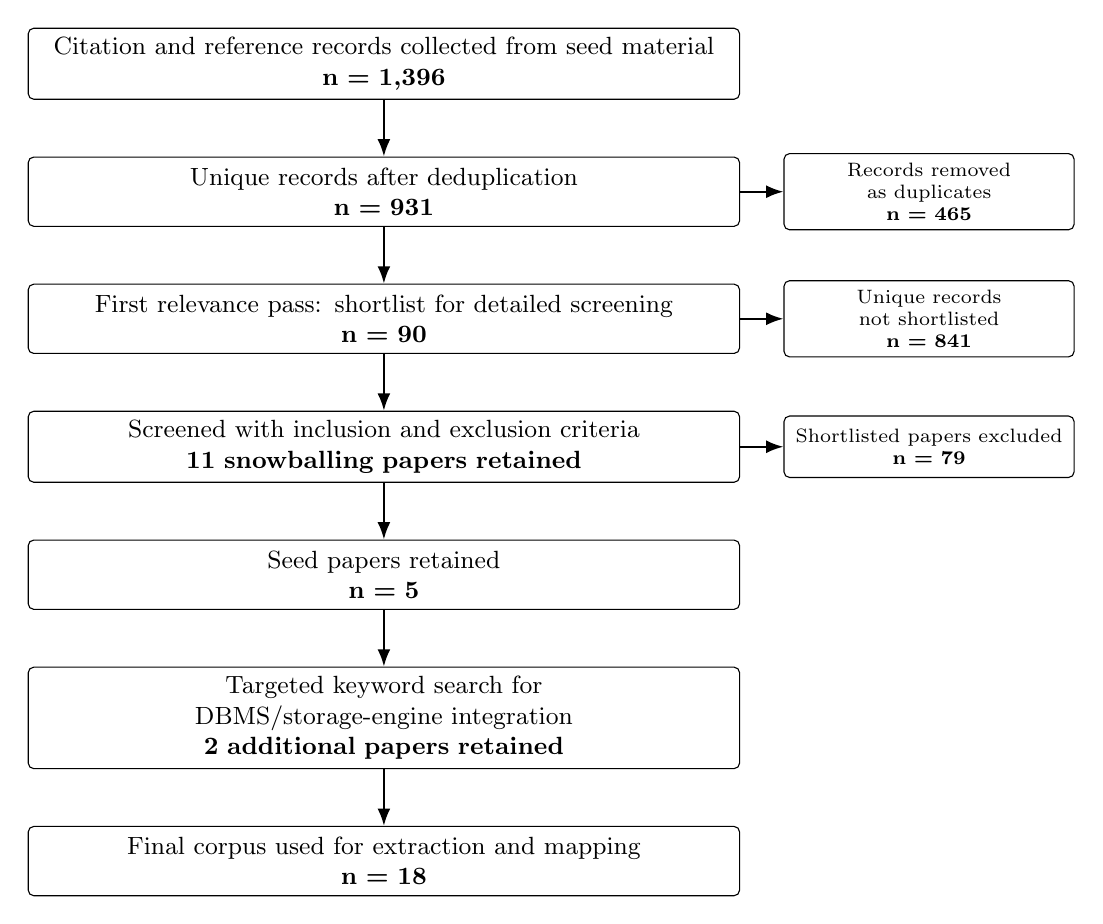
\begin{tikzpicture}[
  node distance=0.72cm,
  box/.style={rectangle, draw=black, rounded corners=2pt, align=center, text width=8.8cm, minimum height=0.88cm, font=\small},
  sidebox/.style={rectangle, draw=black, rounded corners=2pt, align=center, text width=3.45cm, minimum height=0.78cm, font=\scriptsize},
  arrow/.style={-{Latex[length=2.2mm]}, thick}
]
\node[box] (raw) {Citation and reference records collected from seed material\\\textbf{n = 1,396}};
\node[box, below=of raw] (dedup) {Unique records after deduplication\\\textbf{n = 931}};
\node[box, below=of dedup] (shortlist) {First relevance pass: shortlist for detailed screening\\\textbf{n = 90}};
\node[box, below=of shortlist] (screened) {Screened with inclusion and exclusion criteria\\\textbf{11 snowballing papers retained}};
\node[box, below=of screened] (seeds) {Seed papers retained\\\textbf{n = 5}};
\node[box, below=of seeds] (targeted) {Targeted keyword search for DBMS/storage-engine integration\\\textbf{2 additional papers retained}};
\node[box, below=of targeted] (final) {Final corpus used for extraction and mapping\\\textbf{n = 18}};

\node[sidebox, right=0.55cm of dedup] (dups) {Records removed as duplicates\\\textbf{n = 465}};
\node[sidebox, right=0.55cm of shortlist] (notshort) {Unique records not shortlisted\\\textbf{n = 841}};
\node[sidebox, right=0.55cm of screened] (excluded) {Shortlisted papers excluded\\\textbf{n = 79}};

\draw[arrow] (raw) -- (dedup);
\draw[arrow] (dedup) -- (shortlist);
\draw[arrow] (shortlist) -- (screened);
\draw[arrow] (screened) -- (seeds);
\draw[arrow] (seeds) -- (targeted);
\draw[arrow] (targeted) -- (final);
\draw[arrow] (dedup.east) -- (dups.west);
\draw[arrow] (shortlist.east) -- (notshort.west);
\draw[arrow] (screened.east) -- (excluded.west);
\end{tikzpicture}
\caption{PRISMA-style selection flow for the construction of the retained corpus}
\label{fig:selection-flow}
\end{figure}

\newpage
\section{Data Extraction and Classification}

The 18 retained primary papers were analyzed through a common extraction grid. The grid makes the papers comparable and links each extracted element to the research questions.

\begin{longtable}{|p{3.1cm}|p{7.3cm}|p{2.2cm}|}
\hline
\textbf{Group} & \textbf{Extracted data items} & \textbf{Related RQ} \\
\hline
Metadata & paper id, title, authors, year, venue, DOI, source & RQ1 \\
\hline
Publication and contribution & paper type, research type, venue type & RQ1 \\
\hline
Technical focus & index family, classical baselines, data type & RQ2 \\
\hline
Workload and setting & workload type, operating setting, integration context & RQ2 \\
\hline
Evaluation evidence & evaluation type, datasets, metrics, baselines & RQ3 \\
\hline
Reproducibility & code availability, dataset availability, benchmark/framework availability, reproducibility notes & RQ3 \\
\hline
Interpretation & one-sentence summary, main limitations, relevance, inclusion in final analysis & Discussion \\
\hline
\caption{Data extraction grid}
\label{tab:extraction-grid}
\end{longtable}

The classification scheme was refined during extraction. Initial categories were derived from the research questions and the known seed papers. During reading, categories were merged or split when papers made the initial categories too broad. For example, learned-index proposals were separated from benchmarks, critical analyses, tuning methods, and DBMS/storage-engine integration papers. Similarly, the technical focus was separated into families such as RMI/model-based indexes, piecewise linear indexes, adaptive/updatable indexes, disk-resident learned indexes, and DBMS-integrated learned indexes. The label ``hybrid'' is used only for explicit learned/classical combinations.

\section{Tools Used}

Zotero was used to manage references, store PDFs, retrieve metadata, and organize the selected corpus. A spreadsheet was used for selection decisions and data extraction. Markdown files preserved the snowballing trace, including each candidate's source, discovery direction, and relevance notes. The working files were also kept in a private GitHub repository, which made it easier to version the LaTeX source, notes, article lists, and intermediate drafts throughout the project.

\section{Threats to Validity}

This section follows the common SMS practice of making threats explicit rather than treating the map as exhaustive. The threats are grouped by validity type.

\textbf{Descriptive validity.} Descriptive validity concerns whether the selected studies and extracted data were recorded accurately. This threat was mitigated by preserving the source of each candidate, keeping the snowballing trace in Markdown files, managing references in Zotero, and using a common extraction grid. However, extraction was performed by a single reviewer, so mistakes in coding or interpretation remain possible.

\textbf{Theoretical validity.} Theoretical validity concerns whether the search strategy captures the intended research area. Snowballing is sensitive to the initial seed set. To reduce this risk, the five seeds were selected to cover distinct dimensions of learned-index research: foundational RMI work, piecewise/data-aware indexing, adaptive and updatable indexing, cost-based construction, and broad experimental evaluation. A targeted keyword search was also added to reduce the risk of missing DBMS and storage-engine integration papers.

\textbf{Selection validity.} The 90-paper shortlist was selected from 931 unique records. This made the study feasible for an M1 thesis, but it may have excluded relevant papers that were not visible during the first relevance pass. In addition, the backward references of the foundational Kraska et al. paper were not used as primary learned-index candidates. This choice is justified because the paper starts the learned-index research line considered in this thesis, but it may exclude older related work on interpolation search, approximate indexing, or classical access methods from the primary corpus.

\textbf{Interpretive validity.} Interpretive validity concerns whether the conclusions follow from the classifications. The main risk is subjective categorization, especially for papers that combine several roles, such as index proposal, benchmark, tuning method, and DBMS integration. To reduce this risk, the categories were tied to the research questions and the extraction items in Table~\ref{tab:extraction-grid}. The results should therefore be read as a structured map of the selected corpus, not as a definitive ranking of learned-index techniques.

\textbf{External validity.} External validity concerns the generalizability of the map. The corpus focuses on learned indexes in database-system contexts. Its conclusions should not be generalized to all database indexing, classical index advising, vector indexing, text indexing, or spatial indexing. A number of relevant papers are also recent and have limited citation history, particularly papers on DBMS integration, robustness, disk-resident learned indexes, and updatable learned indexes.

\textbf{Reproducibility of evidence.} Reproducibility is uneven across the corpus. Some papers release code, datasets, or benchmarks, while others give only partial implementation details. This variation limits how strongly the mapped evidence can be compared across papers. It is also one of the aspects examined under RQ3.

\chapter{Mapping Results}

This chapter presents the results of the extraction and classification process. The objective is descriptive: the chapter maps what the retained papers study, which techniques and workloads they cover, and what evaluation evidence they provide. It does not rank learned indexes or decide that one structure is universally better than another. This distinction is important because the corpus contains different kinds of contributions: index proposals, benchmark papers, robustness studies, tuning work, and DBMS or storage-engine integration papers.

\section{Overview of the Retained Corpus}

The final corpus contains 18 retained papers. The earliest retained paper is the foundational learned-index proposal by Kraska et al. in 2018 \cite{kraska2018}. The most recent retained paper is PostLearn, a 2026 workshop paper studying learned-index integration in PostgreSQL \cite{fuad2026postlearn}. Between these two points, the corpus expands from standalone learned-index structures toward benchmarking, dynamic updates, disk-resident evaluation, robustness, tuning, and DBMS integration.

Most papers in the corpus study one-dimensional ordered keys and range-index behavior. This is expected because the SMS scope is database-system learned indexes rather than spatial, text, multimedia, vector, or domain-specific indexing. The corpus includes primary learned-index proposals such as FITing-Tree, ALEX, the PGM-index, RadixSpline, CARMI, DILI, and SWIX \cite{galakatos2019fiting,ding2020alex,ferragina2020pgm,kipf2020radixspline,zhang2022carmi,li2023dili,liang2024swix}. It also includes evaluation-centered papers such as SOSD, the comprehensive learned-index evaluation by Sun et al., Are Updatable Learned Indexes Ready?, the critical analysis of RMIs, and the RoBin robustness benchmark \cite{marcus2020benchmarking,sun2023learned,wongkham2022ready,maltry2022critical,luo2025robustness}. A smaller group studies system integration or larger-than-memory settings, including Lan et al.'s disk-resident evaluation, Limousine, LearnedStore, and PostLearn \cite{lan2023disk,chatterjee2024limousine,maharjan2023learnedstore,fuad2026postlearn}.

SageDB was identified during snowballing but was not retained as a primary study because it is broader than learned indexes: it is an instance-optimized analytics DBMS paper in which learned components are part of a wider system vision \cite{ding2022sagedb}. It is therefore used only as contextual related work.

\newpage
\section{RQ1: Publication and Contribution Types}

RQ1 asks what types of learned-index studies have been published, and how they are distributed over time and publication venues. Figure~\ref{fig:year-distribution} summarizes the year distribution in the retained corpus. The zero value for 2021 is kept in the chart to show the gap between the early proposal phase and the later benchmark and robustness phase.

\begin{figure}[h]
\centering
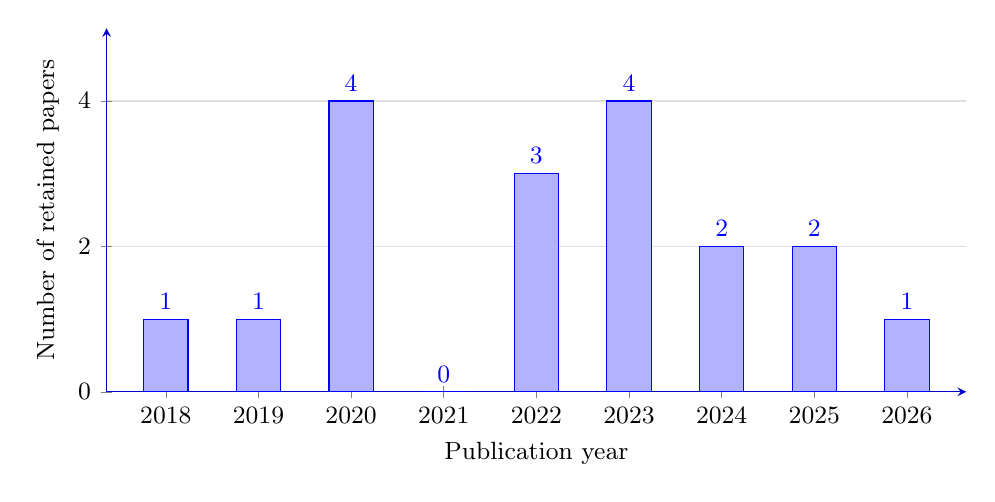
\begin{tikzpicture}
\begin{axis}[
  width=12.5cm,
  height=6.2cm,
  ybar,
  bar width=16pt,
  ymin=0,
  ymax=5,
  ylabel={Number of retained papers},
  xlabel={Publication year},
  symbolic x coords={2018,2019,2020,2021,2022,2023,2024,2025,2026},
  xtick=data,
  nodes near coords,
  nodes near coords align={vertical},
  every node near coord/.append style={font=\small},
  axis lines=left,
  ymajorgrids=true,
  grid style={gray!25},
  tick label style={font=\small},
  label style={font=\small},
  enlarge x limits=0.08,
  fill=bleuleger!45,
  draw=bleuleger
]
\addplot coordinates {(2018,1) (2019,1) (2020,4) (2021,0) (2022,3) (2023,4) (2024,2) (2025,2) (2026,1)};
\end{axis}
\end{tikzpicture}
\caption{Year distribution of the 18 retained primary studies}
\label{fig:year-distribution}
\end{figure}

The time distribution shows three phases. The first phase starts with the original RMI proposal and early learned-index structures \cite{kraska2018,galakatos2019fiting}. The second phase, around 2020--2022, broadens the field with dynamic learned indexes, compressed and piecewise-linear indexes, cache-aware construction, and systematic benchmarking \cite{ding2020alex,ferragina2020pgm,kipf2020radixspline,marcus2020benchmarking,zhang2022carmi,wongkham2022ready,maltry2022critical}. The third phase, from 2023 onward, shifts more attention toward practical limitations: disk-resident behavior, robustness, tuning, streaming windows, larger-than-memory storage engines, and DBMS integration \cite{lan2023disk,sun2023learned,li2023dili,maharjan2023learnedstore,liang2024swix,chatterjee2024limousine,wang2025tuning,luo2025robustness,fuad2026postlearn}.

The venue distribution is concentrated in database venues and database-adjacent workshops. Several retained papers appear in SIGMOD or Proceedings of the ACM on Management of Data \cite{kraska2018,galakatos2019fiting,ding2020alex,lan2023disk,liang2024swix,chatterjee2024limousine,wang2025tuning,luo2025robustness}. Several others are published in Proceedings of the VLDB Endowment \cite{marcus2020benchmarking,ferragina2020pgm,maltry2022critical,zhang2022carmi,wongkham2022ready,sun2023learned,li2023dili}. The remaining retained papers include workshop or other conference publications \cite{kipf2020radixspline,maharjan2023learnedstore,fuad2026postlearn}. This confirms that the selected corpus is mainly located in the database-systems literature rather than in general machine learning venues.

Table~\ref{tab:contribution-types} maps the main contribution types. Several papers fit more than one label; for example, Lan et al. is both a disk-resident evaluation and a source of design choices for future on-disk learned indexes, while Maltry and Dittrich is both a critical analysis and a tuning-oriented RMI study \cite{lan2023disk,maltry2022critical}. For this reason, the table reports dominant roles rather than mutually exclusive categories.

\begin{table}[h]
\begin{center}
\begin{tabular}{|p{4cm}|p{2cm}|p{7cm}|}
\hline
\textbf{Dominant contribution type} & \textbf{Count} & \textbf{Examples} \\
\hline
Index proposal or index design & 8 & RMI, FITing-Tree, ALEX, PGM-index, RadixSpline, CARMI, DILI, SWIX \cite{kraska2018,galakatos2019fiting,ding2020alex,ferragina2020pgm,kipf2020radixspline,zhang2022carmi,li2023dili,liang2024swix} \\
\hline
Benchmark or critical evaluation & 5 & SOSD, Sun et al., Are Updatable Learned Indexes Ready?, Critical Analysis of RMIs, RoBin \cite{marcus2020benchmarking,sun2023learned,wongkham2022ready,maltry2022critical,luo2025robustness} \\
\hline
DBMS, storage-engine, or larger-than-memory integration & 4 & Lan et al., Limousine, LearnedStore, PostLearn \cite{lan2023disk,chatterjee2024limousine,maharjan2023learnedstore,fuad2026postlearn} \\
\hline
Tuning method & 1 & LITune \cite{wang2025tuning} \\
\hline
\end{tabular}
\end{center}
\caption{Dominant contribution types in the retained corpus}
\label{tab:contribution-types}
\end{table}

Figure~\ref{fig:contribution-setting-bubble} cross-checks contribution type with the primary system setting used in the retained papers. The largest bubbles confirm that most index proposals and benchmark papers are still standalone or in-memory studies, while the system-integration papers are split between disk-resident, storage-engine, and DBMS settings.

\begin{figure}[h]
\centering
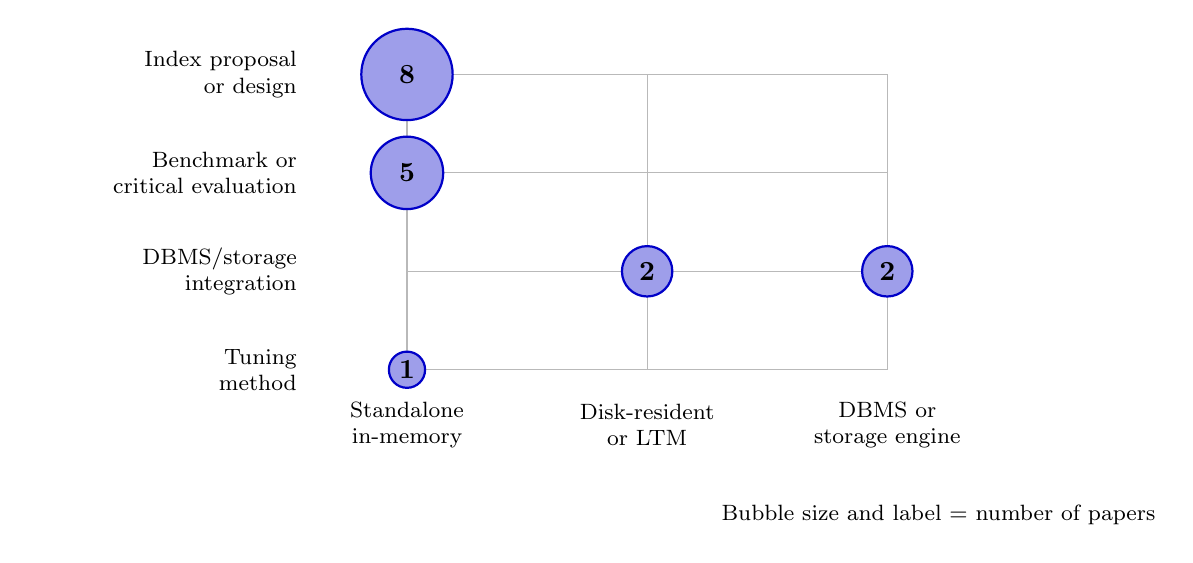
\begin{tikzpicture}[font=\small]
\def\xgap{3.05}
\def\ygap{1.25}

\foreach \x/\label in {1/{Standalone\\in-memory},2/{Disk-resident\\or LTM},3/{DBMS or\\storage engine}} {
  \node[align=center, font=\footnotesize] at (\x*\xgap,0.55) {\label};
}
\foreach \y/\label in {1/{Tuning\\method},2/{DBMS/storage\\integration},3/{Benchmark or\\critical evaluation},4/{Index proposal\\or design}} {
  \node[align=right, font=\footnotesize, text width=3.3cm] at (0,\y*\ygap) {\label};
}

\draw[gray!55] (1*\xgap,1*\ygap) grid[xstep=\xgap,ystep=\ygap] (3*\xgap,4*\ygap);
\draw[gray!55] (1*\xgap,1*\ygap) rectangle (3*\xgap,4*\ygap);

\foreach \x/\y/\r/\n in {
  1/4/0.58/8,
  1/3/0.46/5,
  2/2/0.32/2,
  3/2/0.32/2,
  1/1/0.23/1
} {
  \filldraw[fill=bleuleger!38, draw=bleuleger, line width=0.8pt] (\x*\xgap,\y*\ygap) circle (\r);
  \node[font=\bfseries] at (\x*\xgap,\y*\ygap) {\n};
}

\node[align=left, font=\footnotesize] at (9.8,-0.6) {Bubble size and label = number of papers};
\end{tikzpicture}
\caption{Bubble plot of dominant contribution type by primary system setting in the retained corpus}
\label{fig:contribution-setting-bubble}
\end{figure}

The map shows that learned-index research is no longer only a sequence of new index structures. New structures remain important, but a large part of the recent corpus studies whether these structures remain effective under broader evaluation conditions. This is visible in the movement from RMI and FITing-Tree-style proposals toward benchmark and robustness papers that compare multiple learned and traditional indexes under common workloads \cite{kraska2018,galakatos2019fiting,marcus2020benchmarking,sun2023learned,wongkham2022ready,luo2025robustness}.

\section{RQ2: Techniques, Workloads, and System Settings}

RQ2 asks which learned-index techniques and database workload scenarios are addressed in the literature. Table~\ref{tab:technical-map} summarizes the main technical families found in the corpus.

\begin{longtable}{|p{3.1cm}|p{7.7cm}|p{1.8cm}|}
\hline
\textbf{Technical family} & \textbf{Representative retained papers} & \textbf{Level} \\
\hline
RMI and model-based learned indexes & Kraska et al., ALEX, CARMI, RMI analysis, LearnedStore \cite{kraska2018,ding2020alex,zhang2022carmi,maltry2022critical,maharjan2023learnedstore} & High \\
\hline
Piecewise linear and bounded-error learned indexes & FITing-Tree, PGM-index, RadixSpline, DILI, SWIX \cite{galakatos2019fiting,ferragina2020pgm,kipf2020radixspline,li2023dili,liang2024swix} & High \\
\hline
Adaptive or updatable learned indexes & ALEX, PGM-index, CARMI, DILI, SWIX, Wongkham et al., Sun et al., RoBin \cite{ding2020alex,ferragina2020pgm,zhang2022carmi,li2023dili,liang2024swix,wongkham2022ready,sun2023learned,luo2025robustness} & High \\
\hline
Disk-resident or larger-than-memory learned-index studies & Lan et al., Limousine, LearnedStore, PostLearn \cite{lan2023disk,chatterjee2024limousine,maharjan2023learnedstore,fuad2026postlearn} & Medium \\
\hline
Explicit learned/classical combinations & LearnedStore and Limousine \cite{maharjan2023learnedstore,chatterjee2024limousine} & Low \\
\hline
Learned-index tuning & Maltry and Dittrich, LITune \cite{maltry2022critical,wang2025tuning} & Low \\
\hline
\caption{Technical families identified in the corpus}
\label{tab:technical-map}
\end{longtable}

The strongest coverage is for one-dimensional range indexes over ordered keys. The original RMI proposal treats a range index as a learned model of the key-position mapping \cite{kraska2018}. FITing-Tree, PGM-index, RadixSpline, and DILI all continue this broad direction through piecewise linear or distribution-driven approximations \cite{galakatos2019fiting,ferragina2020pgm,kipf2020radixspline,li2023dili}. ALEX, CARMI, and SWIX extend the map toward adaptive layouts, updates, cache-aware construction, and sliding-window behavior \cite{ding2020alex,zhang2022carmi,liang2024swix}.

The workload map is broader than the early learned-index image of read-only lookup, but still uneven. Point lookup is almost universal in the corpus because it is the basic operation used to test key-to-position prediction \cite{kraska2018,marcus2020benchmarking,sun2023learned}. Range queries are also common, especially in learned range indexes such as FITing-Tree, ALEX, PGM-index, CARMI, DILI, SWIX, and the comprehensive benchmark by Sun et al. \cite{galakatos2019fiting,ding2020alex,ferragina2020pgm,zhang2022carmi,li2023dili,liang2024swix,sun2023learned}. Update workloads are covered by ALEX, PGM-index, CARMI, DILI, SWIX, Wongkham et al., Sun et al., Lan et al., and RoBin \cite{ding2020alex,ferragina2020pgm,zhang2022carmi,li2023dili,liang2024swix,wongkham2022ready,sun2023learned,lan2023disk,luo2025robustness}. Concurrent workloads appear in fewer studies, mainly in benchmark or robustness papers and in DBMS-oriented work \cite{wongkham2022ready,sun2023learned,liang2024swix,luo2025robustness,fuad2026postlearn}.

\begin{table}[h]
\begin{center}
\begin{tabular}{|p{3.8cm}|p{8.8cm}|}
\hline
\textbf{Workload category} & \textbf{Coverage in the retained corpus} \\
\hline
Point lookup & Covered by nearly all retained learned-index papers \cite{kraska2018,marcus2020benchmarking,sun2023learned} \\
\hline
Range query & Common in range-index proposals and benchmarks \cite{galakatos2019fiting,ding2020alex,ferragina2020pgm,zhang2022carmi,sun2023learned} \\
\hline
Insert/delete/update & Stronger coverage after ALEX, especially in updatable-index papers and benchmarks \cite{ding2020alex,wongkham2022ready,sun2023learned,li2023dili,luo2025robustness} \\
\hline
Bulk loading & Covered in several proposals and evaluations \cite{galakatos2019fiting,ding2020alex,marcus2020benchmarking,sun2023learned,lan2023disk} \\
\hline
Concurrency & Present but less common than single-threaded lookup and update evaluation \cite{wongkham2022ready,sun2023learned,liang2024swix,luo2025robustness,fuad2026postlearn} \\
\hline
Streaming or sliding-window workloads & Mainly represented by SWIX \cite{liang2024swix} \\
\hline
\end{tabular}
\end{center}
\caption{Workload coverage in the retained corpus}
\label{tab:workload-map}
\end{table}

The system-setting map shows a stronger imbalance. Most retained studies are in-memory evaluations of standalone index structures. This includes the foundational proposal, FITing-Tree, ALEX, PGM-index experiments, RadixSpline, CARMI, DILI, and several benchmark papers \cite{kraska2018,galakatos2019fiting,ding2020alex,ferragina2020pgm,kipf2020radixspline,zhang2022carmi,li2023dili,marcus2020benchmarking,sun2023learned}. This setting is useful for isolating index behavior, but it does not include all DBMS costs.

Fewer papers study disk-resident, storage-engine, or DBMS-integrated settings. Lan et al. explicitly evaluate updatable learned indexes in a disk-resident DBMS-like setting and conclude that in-memory designs cannot simply be transferred to disk without additional design choices \cite{lan2023disk}. LearnedStore integrates a learned model into LeanStore as an accelerator that can jump to likely B+-tree leaf pages while keeping the original B+-tree path as a fallback \cite{maharjan2023learnedstore}. PostLearn integrates an ALEX-derived index into PostgreSQL and shows that learned-index behavior changes when executor overheads, access-method interfaces, and system integration are included \cite{fuad2026postlearn}. Limousine broadens the setting further by combining learned and classical components in larger-than-memory cloud storage-engine design \cite{chatterjee2024limousine}. These papers make DBMS integration visible, but they remain a minority compared with standalone in-memory evaluations.

\section{RQ3: Evaluation Evidence and Reproducibility}

RQ3 asks how learned indexes are evaluated and what evidence is available regarding performance, robustness, and reproducibility. The dominant evaluation type is experimental benchmarking. Nearly all retained papers report experiments, either for a proposed index or for a comparative benchmark. Common metrics include lookup latency, throughput, memory footprint, build time, update cost, range-query cost, prediction error, tail latency, and sometimes hardware-level behavior such as cache misses or branch misses \cite{marcus2020benchmarking,sun2023learned,wongkham2022ready,lan2023disk,luo2025robustness}.

The most common baselines are B+-tree variants, Adaptive Radix Tree, binary search variants, and other learned indexes. The foundational proposal compares against cache-optimized B-trees, FAST, lookup tables, hash structures, and Bloom filters depending on the index type being studied \cite{kraska2018}. SOSD compares learned indexes against B-tree-like structures, ART, FAST, FST, Wormhole, hash-based structures, binary search, and radix binary search \cite{marcus2020benchmarking}. Later benchmark papers extend this style by comparing multiple learned indexes against B+tree, ART, Wormhole, Masstree, HOT, and concurrent variants \cite{wongkham2022ready,sun2023learned,luo2025robustness}. This indicates that the evaluation culture of the field has become increasingly comparative rather than limited to single-paper baselines.

Datasets are also increasingly standardized. Many papers use SOSD-style datasets such as Amazon Books, Facebook user IDs, OpenStreetMap, and Wikipedia timestamps \cite{marcus2020benchmarking,kipf2020radixspline,maltry2022critical,sun2023learned,li2023dili,liang2024swix}. Other papers use Weblogs, IoT or MgBench timestamps, YCSB-derived keys, synthetic uniform/lognormal/Zipf/normal distributions, PostgreSQL synthetic relations, LeanStore-style synthetic and real datasets, or data from cloud and storage-engine studies \cite{kraska2018,galakatos2019fiting,ferragina2020pgm,ding2020alex,zhang2022carmi,lan2023disk,maharjan2023learnedstore,chatterjee2024limousine,fuad2026postlearn}. The repeated use of SOSD datasets makes some comparisons easier, but the corpus still contains many differences in hardware, implementation, tuning, workload mix, and integration level.

\begin{longtable}{|p{4cm}|p{8.8cm}|}
\hline
\textbf{Evidence dimension} & \textbf{Observed pattern} \\
\hline
Performance metrics & Lookup latency and throughput are the most common; memory and build time are also frequent \cite{marcus2020benchmarking,sun2023learned}. \\
\hline
Dynamic-workload metrics & Update cost, mixed workload throughput, range-query cost, and tail latency appear mainly in updatable and robustness studies \cite{ding2020alex,wongkham2022ready,lan2023disk,luo2025robustness}. \\
\hline
Robustness evidence & Stronger in benchmark and critical-analysis papers than in original proposal papers \cite{wongkham2022ready,sun2023learned,luo2025robustness}. \\
\hline
Baselines & B+-tree variants, ART, binary search, FAST, Wormhole, and other learned indexes are recurring baselines \cite{kraska2018,marcus2020benchmarking,sun2023learned}. \\
\hline
Datasets & SOSD datasets are recurring, but papers also use synthetic, YCSB, OpenStreetMap, Weblogs, PostgreSQL, LeanStore, and private or system-specific datasets \cite{marcus2020benchmarking,lan2023disk,maharjan2023learnedstore,fuad2026postlearn}. \\
\hline
Artifact availability & Public code and datasets are common in benchmark-centered papers, but less consistent in DBMS integration and broader system papers \cite{marcus2020benchmarking,wongkham2022ready,sun2023learned,lan2023disk,luo2025robustness,fuad2026postlearn}. \\
\hline
\caption{Evaluation evidence mapped under RQ3}
\label{tab:evaluation-map}
\end{longtable}

Reproducibility evidence is mixed. Several papers provide explicit public artifacts or artifact statements. SOSD provides an open benchmark and dataset infrastructure, including an author-verified RMI implementation and an official/tuned FITing-Tree implementation used for comparative evaluation \cite{marcus2020benchmarking,kraska2018,galakatos2019fiting}. The PGM-index, RadixSpline, Maltry and Dittrich's RMI analysis, Sun et al.'s learned-index testbed, Wongkham et al.'s evaluation, SWIX, DILI, Lan et al.'s disk experiment, and RoBin all report public code, benchmark, or implementation artifacts in the extracted evidence \cite{ferragina2020pgm,kipf2020radixspline,maltry2022critical,sun2023learned,wongkham2022ready,liang2024swix,li2023dili,lan2023disk,luo2025robustness}. These papers make the field more reproducible than a collection of isolated prototypes.

However, artifact support is not uniform. Even when public implementations exist through later benchmark infrastructure, original papers may still rely on proprietary or reconstructed datasets, partial implementation details, or separate tuning choices. Several integration-oriented studies are harder to reproduce completely because they depend on system modifications, private data, specific storage-engine configurations, cloud-cost assumptions, or prototype code that is not clearly released in the paper evidence \cite{chatterjee2024limousine,fuad2026postlearn}. This matters for the interpretation of results: standalone benchmark results are easier to compare than DBMS-integration results, but DBMS-integration results may be closer to deployment constraints.

The extracted limitations also form part of the evidence map. Early learned-index results are often strongest under read-heavy, in-memory, distribution-friendly workloads \cite{marcus2020benchmarking}. Updatable learned indexes improve the scope of the field, but benchmark and robustness papers show that write-heavy workloads, hard-to-model datasets, concurrent execution, tail latency, and memory overhead remain challenging \cite{wongkham2022ready,sun2023learned,luo2025robustness}. Disk-resident and DBMS-integrated papers show another limitation: an index that performs well as a standalone structure may lose part of its advantage once persistence, page layout, executor overhead, optimizer interaction, logging, or fallback behavior enters the design \cite{lan2023disk,maharjan2023learnedstore,fuad2026postlearn}.

\section{Summary of the Map}

The mapping results answer the three research questions as follows. For RQ1, the corpus shows a progression from foundational learned-index proposals toward benchmarks, robustness studies, tuning, and system integration. The retained literature is concentrated in database venues, especially SIGMOD/PACMMOD, PVLDB, and database workshops.

For RQ2, the best-covered technical area is one-dimensional ordered indexing, especially RMI-style, piecewise-linear, adaptive, and updatable learned indexes. Lookup and range workloads are well represented; inserts and mixed workloads are increasingly represented; concurrency, streaming, disk-resident execution, and full DBMS integration are present but less common. The narrow learned/classical hybrid category is represented mainly by LearnedStore and Limousine \cite{maharjan2023learnedstore,chatterjee2024limousine}.

For RQ3, the evidence base is experimental and comparative, with increasing use of common benchmarks, strong baselines, and public artifacts. At the same time, reproducibility and comparability remain uneven because papers differ in workload assumptions, datasets, tuning effort, system setting, and artifact availability. The map therefore supports a cautious interpretation: learned indexes are an active database-systems research area with strong evidence for selected settings, but the literature still contains visible gaps around robust dynamic behavior, disk-resident operation, concurrency, and integration into complete DBMSs.

\chapter{Discussion}

The mapping results point to a cautious reading of the learned-index literature. The field has moved beyond the original idea of replacing classical indexes with learned models. Learned indexes can be useful under specific workload and data conditions, but their practical value depends on update behavior, robustness, integration cost, and reproducibility evidence.

\section{From Replacement Claims to Conditional Design Space}

The first visible trend is a shift in how learned indexes are framed. The original proposal made a strong conceptual claim: indexes can be treated as models, and a learned model can replace or reduce parts of traditional access structures by predicting key positions \cite{kraska2018}. Early index proposals such as FITing-Tree, the PGM-index, RadixSpline, ALEX, and CARMI then explored different ways to make this idea practical through bounded-error segments, recursive models, cache-aware construction, dynamic layouts, or single-pass construction \cite{galakatos2019fiting,ferragina2020pgm,kipf2020radixspline,ding2020alex,zhang2022carmi}.

The mapping shows, however, that the field no longer treats learned indexes mainly as universal replacements for B+-trees. Benchmark and critical-analysis papers repeatedly report that performance depends on data distribution, workload mix, implementation quality, tuning, and baseline strength \cite{marcus2020benchmarking,sun2023learned,wongkham2022ready,maltry2022critical,luo2025robustness}. The strongest results usually come from specific settings, especially read-heavy and in-memory workloads over data distributions that are easier to model. This places learned indexes inside a conditional design space rather than a simple replacement story.

This shift is clearest in the benchmark literature. SOSD showed that learned indexes can be highly competitive for read-only in-memory lookup on real datasets, while also emphasizing the need for open implementations, strong baselines, and common datasets \cite{marcus2020benchmarking}. Sun et al. broadened the comparison across lookups, ranges, updates, concurrency, strings, and bulk loading, showing that different learned indexes win under different conditions \cite{sun2023learned}. Wongkham et al. and Luo et al. then made robustness a central question, showing that updatable learned indexes can lose their advantage under hard datasets, skewed inserts, concurrency, tail-latency constraints, or memory pressure \cite{wongkham2022ready,luo2025robustness}. Recent work is therefore less focused on proposing one more learned index and more focused on understanding when these structures actually hold up.

\section{Workload Coverage and Remaining Blind Spots}

The workload map in Table~\ref{tab:workload-map} indicates strong coverage of point lookup and substantial coverage of range queries. This is expected because the learned range-index idea is built around predicting positions in sorted data \cite{kraska2018}. It is also why many retained papers use one-dimensional numeric keys and SOSD-style datasets: these settings make the key-to-position mapping clear and allow indexes to be compared under controlled conditions \cite{marcus2020benchmarking,sun2023learned}.

The corpus also shows increasing attention to dynamic workloads. ALEX, the PGM-index, CARMI, DILI, and SWIX all address updates or changing data in different ways \cite{ding2020alex,ferragina2020pgm,zhang2022carmi,li2023dili,liang2024swix}. Benchmark papers further evaluate inserts, deletes, mixed workloads, and bulk loading \cite{wongkham2022ready,sun2023learned,luo2025robustness}. This means that it would be inaccurate to describe learned-index research as purely static or read-only.

At the same time, dynamic behavior is not solved uniformly. Update support is often evaluated in specific in-memory settings, while concurrent execution, tail latency, skewed inserts, and long-running workload shifts are less consistently studied \cite{wongkham2022ready,luo2025robustness}. SWIX is an important exception for sliding-window and streaming workloads, but it also illustrates that specialized workload assumptions can produce specialized designs rather than general-purpose DBMS indexes \cite{liang2024swix}. Future learned-index evaluations need more than average lookup speed: they also need to show what happens after sustained updates, changing distributions, concurrent operations, and mixed read/write phases.

Range-query evidence also requires nuance. Learned indexes can locate the start of a range efficiently, but range performance then depends on layout, scan efficiency, gaps, leaf organization, and payload access. ALEX reports strong support for short ranges, while PostLearn reports that PostgreSQL's B+-tree becomes faster for larger ranges in its experiment because scanning packed leaf pages is more efficient than scanning ALEX+'s gapped arrays with bitmap checks \cite{ding2020alex,fuad2026postlearn}. Wongkham et al. similarly show that learned indexes do not generally dominate traditional indexes for range-heavy workloads \cite{wongkham2022ready}. Future studies should separate short ranges, long ranges, covering scans, secondary-index scans, and DBMS tuple-fetching costs, because these cases may lead to different conclusions.

\section{DBMS Integration as a Major Evidence Gap}

The strongest imbalance in the map is the difference between standalone in-memory evaluation and full database-system integration. Most retained papers evaluate index structures in isolation. This is useful because it isolates the algorithmic behavior of the index, but it also leaves out DBMS concerns such as disk layout, buffer behavior, query execution overhead, optimizer interaction, tuple visibility checks, concurrency control, and persistence \cite{lan2023disk,fuad2026postlearn}.

The smaller group of integration-oriented papers is especially important. Lan et al. show that moving updatable learned indexes into disk-resident settings creates design constraints that are not visible in memory-only experiments \cite{lan2023disk}. LearnedStore takes a hybrid approach by using a learned model as an accelerator for LeanStore's B+-tree search rather than replacing the B+-tree entirely \cite{maharjan2023learnedstore}. PostLearn integrates an ALEX-derived index into PostgreSQL and shows that standalone index speedups can shrink once relational executor overhead and DBMS access-method interfaces are included \cite{fuad2026postlearn}. Limousine broadens the discussion further by treating learned and classical components as parts of a larger cloud storage-engine design space \cite{chatterjee2024limousine}.

These papers suggest a practical interpretation: the most deployable learned-index designs may be hybrid or system-aware. LearnedStore preserves the B+-tree fallback path, which reduces the risk of bad model predictions or distribution shifts \cite{maharjan2023learnedstore}. Limousine explicitly blends learned and classical components across storage-engine designs \cite{chatterjee2024limousine}. This is consistent with the original RMI paper's own observation that weak learned models can be replaced by B-trees in parts of the hierarchy \cite{kraska2018}. In practice, learned indexes may be most useful as components that accelerate selected paths in a storage engine.

This gap also affects external validity. PostLearn shows that a standalone ALEX+ speedup becomes smaller inside PostgreSQL because the relational execution path adds overheads such as executor work and MVCC visibility checks \cite{fuad2026postlearn}. Lan et al. similarly show that disk-resident learned indexes face design constraints that are not visible in in-memory tests \cite{lan2023disk}. Conversely, a learned component may still be valuable if it reduces memory, cloud cost, or search depth inside a larger system \cite{chatterjee2024limousine}. More end-to-end evaluations are needed, especially inside existing DBMSs or storage engines, with both index-level and query-level results.

\section{Robustness, Tuning, and the Cost of Practical Use}

Learned indexes also introduce a practical tuning burden. Model architecture, segment size, error bounds, node layout, update thresholds, search strategy, and workload assumptions can all affect performance. Maltry and Dittrich show this clearly for RMIs: a more accurate model is not automatically faster if model evaluation becomes expensive or if correction search remains costly \cite{maltry2022critical}. CARMI uses cost-based construction to improve cache-aware behavior, and LITune later applies reinforcement learning to tune learned-index parameters under static and changing workloads \cite{zhang2022carmi,wang2025tuning}.

This tuning literature is important because it changes the interpretation of performance results. A learned index may perform well when carefully tuned by its authors, but practitioners need methods for choosing parameters under their own datasets and workloads. Benchmarks such as SOSD and Sun et al.'s testbed reduce this problem by providing common implementations and evaluation settings \cite{marcus2020benchmarking,sun2023learned}. However, benchmark standardization does not remove the need for workload-specific tuning, especially for adaptive and updatable learned indexes.

Robustness papers further show that performance regressions can come from model overfitting, unbalanced structures, structural modification heuristics, excessive space reservation, and difficult insert patterns \cite{luo2025robustness}. These are not minor engineering details; they directly affect whether learned indexes can be trusted in database systems. Tail latency, memory growth, rebuild cost, and failure under corner-case distributions deserve the same attention as average lookup latency.

Learned-index papers should show more clearly how stable their results are when the setup changes. Useful evidence would include parameter sweeps, workload-shift experiments, update histories, tail-latency distributions, and negative cases where the learned index is not competitive. This would make the literature more useful for practitioners and would also make results easier to compare.

\section{Reproducibility and Comparability}

Several retained studies provide public code, datasets, or benchmark frameworks. SOSD is central in this respect because it introduced common datasets and a benchmark environment for learned-index comparison \cite{marcus2020benchmarking}. Later papers such as the PGM-index, RadixSpline, CARMI, Maltry and Dittrich's RMI analysis, Sun et al.'s testbed, Wongkham et al.'s benchmark, DILI, SWIX, Lan et al.'s disk-resident evaluation, and RoBin all report public code or artifact evidence in the extracted data \cite{ferragina2020pgm,kipf2020radixspline,zhang2022carmi,maltry2022critical,sun2023learned,wongkham2022ready,li2023dili,liang2024swix,lan2023disk,luo2025robustness}.

Nevertheless, reproducibility remains uneven. Some original papers rely on proprietary, private, or reconstructed datasets; some DBMS-integration studies depend on prototype modifications that are harder to reproduce; and some system-level evaluations include cloud settings, cost models, or configuration choices that are not as easy to rerun as standalone lookup benchmarks \cite{chatterjee2024limousine,fuad2026postlearn}. Artifact availability is therefore not a binary quality label. A paper can provide enough detail to understand its design while still being difficult to reproduce fully.

Comparability is also limited by differences in baseline selection and tuning effort. A weakly tuned B+-tree or ART baseline can exaggerate learned-index gains, while a weak learned-index implementation can hide them. SOSD and later benchmark papers explicitly address this problem by using stronger baselines and shared implementations \cite{marcus2020benchmarking,sun2023learned}. Learned-index papers should justify baseline choice, report tuning procedures for both learned and classical indexes, and make clear whether comparisons are index-level microbenchmarks or DBMS-level experiments.

\section{Relation to Existing Surveys}

Existing surveys answer different questions from this thesis. Faraj and Ali provide a narrative survey and taxonomy of learned-index techniques \cite{faraj2024survey}. Liu et al. provide an experimental survey of multi-dimensional learned indexes, and Al-Mamun et al. survey learned indexes for multi-dimensional space \cite{liu2025multidimensional,almamun2025survey}.

This study has a different role. It maps primary studies in database-system learned indexing through explicit research questions, inclusion and exclusion criteria, snowballing and targeted search, and a common extraction grid. For that reason, the discussion emphasizes publication type, workload coverage, system setting, evaluation practice, and reproducibility. Multi-dimensional learned-index surveys are treated as related work because their scope differs from the one-dimensional ordered-index literature that dominates the retained primary studies.

\section{Implications for Future Research}

Five research gaps stand out. First, more work is needed on disk-resident and DBMS-integrated learned indexes. PostLearn and LearnedStore are important steps, but the literature still lacks broad evidence across mature DBMSs, persistent storage layouts, optimizer cost models, recovery mechanisms, and transactional updates \cite{maharjan2023learnedstore,fuad2026postlearn}.

Second, learned-index robustness should remain a central evaluation topic. Future proposals should test hard distributions, outliers, skewed inserts, concurrent workloads, long-running update histories, and distribution shifts rather than relying mainly on favorable read-heavy settings \cite{wongkham2022ready,luo2025robustness}.

Third, hybrid learned/classical designs deserve more systematic study. LearnedStore and Limousine suggest that learned components may be most useful when combined with classical fallbacks, page structures, buffers, or storage-engine design choices \cite{maharjan2023learnedstore,chatterjee2024limousine}. The map contains only a small number of such papers, so this remains an underdeveloped area.

Fourth, future evaluations should report more complete cost models. Lookup latency alone is insufficient. Memory footprint, build time, retraining time, update cost, tail latency, parameter-tuning cost, cloud cost, and operational complexity can change the practical conclusion \cite{marcus2020benchmarking,maltry2022critical,wang2025tuning,chatterjee2024limousine}.

Fifth, artifact support should be treated as part of the research contribution. The strongest benchmark papers improved the field by reporting results and by making comparison easier for later work \cite{marcus2020benchmarking,sun2023learned,wongkham2022ready}. More DBMS-integration papers with public prototypes, reproducible workloads, and clear configuration scripts would make the next generation of mapping or systematic review more precise. A broader long-term direction could be the move toward instance-optimized or self-designing DBMSs; SageDB illustrates this system-level vision, and learned indexes could become one of the physical-design components needed for such systems when data distributions and workloads make them appropriate \cite{ding2022sagedb}.

\section{Summary}

Overall, learned-index research has produced a substantial body of index proposals, benchmarks, robustness studies, tuning methods, and early system-integration work. The evidence is strongest for one-dimensional in-memory ordered-key workloads, especially lookup-oriented evaluations. The evidence is weaker, but growing, for disk-resident execution, full DBMS integration, concurrency, long-running updates, hybrid learned/classical designs, and reproducible system-level artifacts. The field is best understood as an active design space where learned components can be valuable when their assumptions match the workload and system context.

\chapter{Conclusion}

This thesis conducted a Systematic Mapping Study of learned indexes in database-system contexts. The objective was to classify the literature by contribution type, technical focus, workload and system setting, evaluation practice, and reproducibility evidence. This framing follows the role of an SMS as a method for structuring a heterogeneous research area and identifying research clusters and gaps \cite{petersen2008,petersen2015}. The study used five seed papers, backward and forward snowballing, a targeted search for DBMS and storage-engine integration papers, explicit inclusion and exclusion criteria, and a common extraction grid. The final corpus contains 18 primary studies.

For RQ1, the map shows a field that has diversified since the original learned-index proposal. The earliest retained papers focus on learned-index structures, starting with RMI and followed by designs such as FITing-Tree, ALEX, the PGM-index, RadixSpline, and CARMI \cite{kraska2018,galakatos2019fiting,ding2020alex,ferragina2020pgm,kipf2020radixspline,zhang2022carmi}. Later papers expand the field toward benchmark infrastructure, critical analysis, robustness, tuning, disk-resident behavior, and integration into storage engines or DBMSs \cite{marcus2020benchmarking,maltry2022critical,wongkham2022ready,sun2023learned,lan2023disk,chatterjee2024limousine,wang2025tuning,luo2025robustness,maharjan2023learnedstore,fuad2026postlearn}. The retained literature is concentrated in database venues, especially SIGMOD/PACMMOD, PVLDB, and database-oriented workshops. This indicates a maturing database-systems research topic with a growing emphasis on evaluation, robustness, and integration.

For RQ2, the strongest coverage is one-dimensional ordered indexing. The main technical families are RMI or model-based learned indexes, piecewise linear indexes with bounded errors, adaptive or updatable learned indexes, and a smaller group of system-integrated or explicit learned/classical combinations \cite{kraska2018,galakatos2019fiting,ferragina2020pgm,kipf2020radixspline,ding2020alex,zhang2022carmi,li2023dili,liang2024swix,maharjan2023learnedstore,chatterjee2024limousine}. Point lookups and range queries are well represented. Inserts, deletes, mixed workloads, and bulk loading receive increasing attention through updatable learned indexes and benchmark papers \cite{ding2020alex,wongkham2022ready,sun2023learned,li2023dili,luo2025robustness}. Coverage is thinner for concurrency, streaming or sliding-window workloads, disk-resident execution, larger-than-memory storage, and full DBMS integration \cite{liang2024swix,lan2023disk,chatterjee2024limousine,fuad2026postlearn}.

For RQ3, the evidence base is mainly experimental and comparative. Common metrics include lookup latency, throughput, memory footprint, build or training time, update cost, range-query cost, robustness, and sometimes cache or branch behavior \cite{marcus2020benchmarking,sun2023learned,wongkham2022ready,lan2023disk,luo2025robustness}. Common baselines include B+-tree variants, Adaptive Radix Tree, binary search variants, FAST, Wormhole, hash-based structures, and other learned indexes \cite{kraska2018,marcus2020benchmarking,sun2023learned}. SOSD-style datasets and reusable benchmark frameworks improve comparability, and several retained papers provide public code or artifacts \cite{marcus2020benchmarking,sun2023learned,wongkham2022ready,liang2024swix,luo2025robustness}. At the same time, comparison remains difficult because papers differ in workload mix, tuning effort, hardware, datasets, implementation maturity, and system setting. Artifact evidence is also less consistent for integration-oriented and broader system papers \cite{chatterjee2024limousine,fuad2026postlearn}.

The main finding is therefore cautious. Learned indexes show strong evidence in selected settings, especially read-heavy in-memory workloads over ordered keys where the key distribution can be modeled effectively \cite{kraska2018,marcus2020benchmarking,sun2023learned}. The evidence is weaker for write-heavy workloads, hard-to-model distributions, concurrent access, tail latency, disk-resident operation, and complete DBMS integration \cite{wongkham2022ready,lan2023disk,luo2025robustness,fuad2026postlearn}. The most practically relevant direction in the corpus is increasingly system-aware: learned components may be useful when combined with classical structures, fallback paths, or storage-engine design choices, as illustrated by LearnedStore and Limousine \cite{maharjan2023learnedstore,chatterjee2024limousine}.

This study has limitations. Selection and extraction were performed by a single reviewer, which introduces classification subjectivity. The corpus depends on the five seed papers and on the shortlist constructed from a large snowballing set. The backward references of the original learned-index paper were treated as background rather than candidate learned-index studies because they predate the learned-index literature. The targeted keyword search was intentionally limited to reducing the risk of missing DBMS and storage-engine integration papers. Finally, code and dataset availability were recorded from evidence visible in the papers, so some artifact classifications remain uncertain.

Future work should strengthen the parts of the map that are still underrepresented. The field needs more end-to-end DBMS evaluations, especially under persistence, logging, recovery, optimizer interaction, transactional updates, and mature buffer-management constraints \cite{lan2023disk,fuad2026postlearn}. More evidence is also needed for disk-resident and larger-than-memory workloads, long-running update histories, distribution shifts, concurrency, tail latency, and hybrid learned/classical designs \cite{wongkham2022ready,chatterjee2024limousine,liang2024swix,luo2025robustness}. Reusable artifacts for integration papers would make future comparisons more reliable. Overall, the map shows learned indexes as a condition-dependent database-systems design space: the literature is already strong for several in-memory ordered-key scenarios, while robust and reproducible system-level evidence remains the central challenge for future research.

\renewcommand{\bibname}{Bibliography}
\addcontentsline{toc}{chapter}{Bibliography}
\renewcommand{\refname}{}
\begin{thebibliography}{99}
	   \bibitem{petersen2008}
	   K. Petersen, R. Feldt, S. Mujtaba, and M. Mattsson.
	   Systematic Mapping Studies in Software Engineering.
	   In \textit{Proceedings of the 12th International Conference on Evaluation and Assessment in Software Engineering}, 2008.
	   DOI: 10.14236/ewic/EASE2008.8.

	   \bibitem{petersen2015}
	   K. Petersen, S. Vakkalanka, and L. Kuzniarz.
	   Guidelines for Conducting Systematic Mapping Studies in Software Engineering: An Update.
	   \textit{Information and Software Technology}, 64:1--18, 2015.
	   DOI: 10.1016/j.infsof.2015.03.007.

	   \bibitem{wohlin2014}
	   C. Wohlin.
	   Guidelines for Snowballing in Systematic Literature Studies and a Replication in Software Engineering.
	   In \textit{Proceedings of the 18th International Conference on Evaluation and Assessment in Software Engineering}, 2014.
	   DOI: 10.1145/2601248.2601268.

   \bibitem{kraska2018}
   T. Kraska, A. Beutel, E. H. Chi, J. Dean, and N. Polyzotis.
   The Case for Learned Index Structures.
   In \textit{Proceedings of the 2018 International Conference on Management of Data}, pages 489--504, 2018.
   DOI: 10.1145/3183713.3196909.

   \bibitem{ding2020alex}
   J. Ding, U. F. Minhas, J. Yu, C. Wang, J. Do, Y. Li, H. Zhang, B. Chandramouli, J. Gehrke, D. Kossmann, D. Lomet, and T. Kraska.
   ALEX: An Updatable Adaptive Learned Index.
   In \textit{Proceedings of the 2020 ACM SIGMOD International Conference on Management of Data}, pages 969--984, 2020.
   DOI: 10.1145/3318464.3389711.

   \bibitem{sun2023learned}
   Z. Sun, X. Zhou, and G. Li.
   Learned Index: A Comprehensive Experimental Evaluation.
   \textit{Proceedings of the VLDB Endowment}, 16(8):1992--2004, 2023.
   DOI: 10.14778/3594512.3594528.

   \bibitem{galakatos2019fiting}
   A. Galakatos, M. Markovitch, C. Binnig, R. Fonseca, and T. Kraska.
   FITing-Tree: A Data-aware Index Structure.
   In \textit{Proceedings of the 2019 International Conference on Management of Data}, pages 1189--1206, 2019.
   DOI: 10.1145/3299869.3319860.

   \bibitem{zhang2022carmi}
   J. Zhang and Y. Gao.
   CARMI: A Cache-Aware Learned Index with a Cost-Based Construction Algorithm.
   \textit{Proceedings of the VLDB Endowment}, 15(11):2679--2691, 2022.
   DOI: 10.14778/3551793.3551823.

   \bibitem{marcus2020benchmarking}
   R. Marcus, A. Kipf, A. van Renen, M. Stoian, S. Misra, A. Kemper, T. Neumann, and T. Kraska.
   Benchmarking Learned Indexes.
   \textit{Proceedings of the VLDB Endowment}, 14(1):1--13, 2020.
   DOI: 10.14778/3421424.3421425.

   \bibitem{ding2022sagedb}
   J. Ding, R. Marcus, A. Kipf, V. Nathan, A. Nrusimha, K. Vaidya, A. van Renen, and T. Kraska.
   SageDB: An Instance-Optimized Data Analytics System.
   \textit{Proceedings of the VLDB Endowment}, 15(13):4062--4078, 2022.
   DOI: 10.14778/3565838.3565857.

   \bibitem{lan2023disk}
   H. Lan, Z. Bao, J. S. Culpepper, and R. Borovica-Gajic.
   Updatable Learned Indexes Meet Disk-Resident DBMS: From Evaluations to Design Choices.
   \textit{Proceedings of the ACM on Management of Data}, 1(2):139:1--139:22, 2023.
   DOI: 10.1145/3589284.

   \bibitem{wongkham2022ready}
   C. Wongkham, B. Lu, C. Liu, Z. Zhong, E. Lo, and T. Wang.
   Are Updatable Learned Indexes Ready?
   \textit{Proceedings of the VLDB Endowment}, 15(11):3004--3017, 2022.
   DOI: 10.14778/3551793.3551848.

   \bibitem{chatterjee2024limousine}
   S. Chatterjee, M. F. Pekala, L. Kruglyak, and S. Idreos.
   Limousine: Blending Learned and Classical Indexes to Self-Design Larger-than-Memory Cloud Storage Engines.
   \textit{Proceedings of the ACM on Management of Data}, 2(1):47:1--47:28, 2024.
   DOI: 10.1145/3639302.

   \bibitem{fuad2026postlearn}
   A. Fuad, S. Vashisth, O. Balmau, and B. Kemme.
   PostLearn: Towards A Learned Index For PostgreSQL.
   In \textit{Proceedings of the 6th Workshop on Challenges and Opportunities of Efficient and Performant Storage Systems}, pages 20--25, 2026.
   DOI: 10.1145/3805687.3806257.

   \bibitem{luo2025robustness}
   Y. Luo, M. Xie, Y. Tong, S. Jiang, and Y. Chai.
   Understanding Robustness Issues of Updatable Learned Indexes: Experiments and Analysis.
   \textit{Proceedings of the ACM on Management of Data}, 3(4):270:1--270:25, 2025.
   DOI: 10.1145/3749188.

   \bibitem{maltry2022critical}
   M. Maltry and J. Dittrich.
   A Critical Analysis of Recursive Model Indexes.
   \textit{Proceedings of the VLDB Endowment}, 15(5):1079--1091, 2022.
   DOI: 10.14778/3510397.3510405.

   \bibitem{wang2025tuning}
   T. Wang, L. Liang, G. Yang, T. Heinis, and E. Yoneki.
   A New Paradigm in Tuning Learned Indexes: A Reinforcement Learning Enhanced Approach.
   \textit{Proceedings of the ACM on Management of Data}, 3(3):120:1--120:26, 2025.
   DOI: 10.1145/3725257.

   \bibitem{maharjan2023learnedstore}
   S. Maharjan, S. Zhao, C. Zhong, and S. Jiang.
   From LeanStore to LearnedStore: Using a Learned Index to Improve Database Index Search.
   In \textit{2023 International Conference on High Performance Big Data and Intelligent Systems}, pages 162--169, 2023.
   DOI: 10.1109/HDIS60872.2023.10499467.

   \bibitem{ferragina2020pgm}
   P. Ferragina and G. Vinciguerra.
   The PGM-index: a fully-dynamic compressed learned index with provable worst-case bounds.
   \textit{Proceedings of the VLDB Endowment}, 13(8):1162--1175, 2020.
   DOI: 10.14778/3389133.3389135.

   \bibitem{kipf2020radixspline}
   A. Kipf, R. Marcus, A. van Renen, M. Stoian, A. Kemper, T. Kraska, and T. Neumann.
   RadixSpline: A Single-Pass Learned Index.
   In \textit{Proceedings of the Third International Workshop on Exploiting Artificial Intelligence Techniques for Data Management}, 2020.
   DOI: 10.1145/3401071.3401659.

   \bibitem{li2023dili}
   P. Li, H. Lu, R. Zhu, B. Ding, L. Yang, and G. Pan.
   DILI: A Distribution-Driven Learned Index.
   \textit{Proceedings of the VLDB Endowment}, 16(9):2212--2224, 2023.
   DOI: 10.14778/3598581.3598593.

   \bibitem{liang2024swix}
   L. Liang, G. Yang, A. Hadian, L. A. Croquevielle, and T. Heinis.
   SWIX: A Memory-Efficient Sliding Window Learned Index.
   \textit{Proceedings of the ACM on Management of Data}, 2(1):41:1--41:26, 2024.
   DOI: 10.1145/3639296.

   \bibitem{faraj2024survey}
   C. Q. H. Faraj and N. A. Ali.
   Learned-Indexes for Improving Query Performance: A Comprehensive Survey with Taxonomy.
   \textit{The Scientific Journal of Cihan University - Sulaimaniya}, 8(1):186--209, 2024.
   DOI: 10.25098/8.1.30.

   \bibitem{liu2025multidimensional}
   Q. Liu, M. Li, Y. Zeng, Y. Shen, and L. Chen.
   How Good Are Multi-dimensional Learned Indexes? An Experimental Survey.
   \textit{The VLDB Journal}, 34:17, 2025.
   DOI: 10.1007/s00778-024-00893-6.

   \bibitem{almamun2025survey}
   A. Al-Mamun, H. Wu, Q. He, J. Wang, and W. G. Aref.
   A Survey of Learned Indexes for the Multi-dimensional Space.
   \textit{ACM Computing Surveys}, 58(4):1--37, 2025.
   DOI: 10.1145/3768575.
\end{thebibliography}

\chapter{Appendices}
\appendix
\makeatletter
\def\@seccntformat#1{Appendix~\csname the#1\endcsname:\quad}
\makeatother
\section{Snowballing Trace}

This appendix summarizes the snowballing material used to construct the retained corpus. For each seed paper, citation files were used for forward snowballing and reference files were used for backward snowballing. The only exception is \textit{The Case for Learned Index Structures}: only its citation file was used for primary learned-index candidates because its references predate the learned-index literature considered in this study.

\begin{longtable}{|p{4.4cm}|p{3.5cm}|p{2.2cm}|p{2.2cm}|}
\hline
\textbf{Seed paper} & \textbf{Source file} & \textbf{Direction} & \textbf{Records} \\
\hline
ALEX: An Updatable Adaptive Learned Index & References.md & Backward & 36 \\
\hline
ALEX: An Updatable Adaptive Learned Index & citations.md & Forward & 256 \\
\hline
CARMI: A Cache-Aware Learned Index with a Cost-based Construction Algorithm & citations.md & Forward & 29 \\
\hline
CARMI: A Cache-Aware Learned Index with a Cost-based Construction Algorithm & refrences.md & Backward & 47 \\
\hline
FITing-Tree: A Data-aware Index Structure & citations.md & Forward & 175 \\
\hline
FITing-Tree: A Data-aware Index Structure & refrences.md & Backward & 48 \\
\hline
Learned Index: A Comprehensive Experimental Evaluation & citations.md & Forward & 63 \\
\hline
Learned Index: A Comprehensive Experimental Evaluation & refrences.md & Backward & 28 \\
\hline
The Case for Learned Index Structures & Citations.md & Forward & 714 \\
\hline
\caption{Seed-paper snowballing files and number of records}
\label{tab:appendix-seed-sources}
\end{longtable}

Table~\ref{tab:appendix-retained-trace} reports the retained non-seed papers and their discovery path. The first eleven papers were retained from the snowballing shortlist. The final two papers were added through the targeted keyword search described in Chapter~3. SageDB was identified during snowballing but is treated only as contextual related work because its contribution is broader than learned indexes.

\begin{small}
\begin{longtable}{|p{5.1cm}|p{4.4cm}|p{1.2cm}|p{2.1cm}|}
\hline
\textbf{Retained paper} & \textbf{Found from seed material} & \textbf{Path} & \textbf{Corpus role} \\
\hline
Benchmarking Learned Indexes \cite{marcus2020benchmarking} & CARMI, Learned Index, The Case for Learned Index Structures & B/F & Benchmark \\
\hline
Updatable Learned Indexes Meet Disk-Resident DBMS \cite{lan2023disk} & FITing-Tree & F & Disk evaluation \\
\hline
Are Updatable Learned Indexes Ready? \cite{wongkham2022ready} & ALEX, Learned Index & F/B & Robustness \\
\hline
Limousine: Blending Learned and Classical Indexes \cite{chatterjee2024limousine} & ALEX, FITing-Tree, Learned Index, The Case for Learned Index Structures & F & Storage engine \\
\hline
Understanding Robustness Issues of Updatable Learned Indexes \cite{luo2025robustness} & ALEX, FITing-Tree, Learned Index & F & Robustness \\
\hline
A Critical Analysis of Recursive Model Indexes \cite{maltry2022critical} & Learned Index & B & Critical analysis \\
\hline
A New Paradigm in Tuning Learned Indexes \cite{wang2025tuning} & CARMI, Learned Index & F & Tuning \\
\hline
The PGM-index \cite{ferragina2020pgm} & ALEX, CARMI, FITing-Tree, Learned Index, The Case for Learned Index Structures & B/F & Index design \\
\hline
RadixSpline: A Single-Pass Learned Index \cite{kipf2020radixspline} & FITing-Tree, The Case for Learned Index Structures & F & Index design \\
\hline
DILI: A Distribution-Driven Learned Index \cite{li2023dili} & CARMI, FITing-Tree, The Case for Learned Index Structures & F & Index design \\
\hline
SWIX: A Memory-Efficient Sliding Window Learned Index \cite{liang2024swix} & ALEX & F & Workload \\
\hline
PostLearn: Towards A Learned Index For PostgreSQL \cite{fuad2026postlearn} & Targeted keyword search & Search & DBMS integration \\
\hline
From LeanStore to LearnedStore \cite{maharjan2023learnedstore} & Targeted keyword search & Search & Storage engine \\
\hline
\caption{Trace of retained non-seed papers}
\label{tab:appendix-retained-trace}
\end{longtable}
\end{small}
\end{document}
